\section{Informazioni generali}
\subsection{Definizione di credenziale}
Una credenziale è un insieme di informazioni che serve a identificare una persona o un oggetto. Queste informazioni includono dettagli sul soggetto della credenziale (come una foto, il nome o un numero di identificazione), sull'autorità che l'ha emessa (come un ente governativo o un organismo di certificazione) e sul tipo di credenziale (come un passaporto o una patente di guida). Inoltre, sono presenti informazioni sugli attributi specifici o le caratteristiche che l'autorità afferma riguardo al soggetto (come la nazionalità, le 
categorie di veicoli autorizzate o la data di nascita). La credenziale può anche contenere prove sull'origine della credenziale stessa e restrizioni o vincoli associati (come la data 
di scadenza o i termini d'uso).\\
Una credenziale verificabile rappresenta tutte le stesse informazioni di una credenziale fisica, ma con l'aggiunta di tecnologie come le firme digitali diventa più difficile alterarla e più affidabile. I titolari di credenziali verificabili possono generare presentazioni verificabili per dimostrare di possedere determinate credenziali con specifiche caratteristiche. 
Sia le credenziali verificabili che le presentazioni verificabili possono essere trasmesse rapidamente, rendendole più comode rispetto alle controparti fisiche quando si cerca di 
stabilire la fiducia a distanza.\\
Nonostante questa specifica cerchi di semplificare l'espressione delle credenziali digitali, si fa anche attenzione a preservare la privacy. La persistenza delle informazioni 
digitali e la possibilità di raccogliere e correlare dati provenienti da diverse fonti costituiscono una preoccupazione per la privacy.\\
Il termine "verificabile" nelle credenziali verificabili e nelle presentazioni verificabili si riferisce alla caratteristica di una credenziale o presentazione che può essere 
verificata da un'autorità competente, come definito nel documento. Tuttavia, la verificabilità di una credenziale non implica che la veridicità delle informazioni in essa 
contenute possa essere valutata direttamente. L'emittente può includere nel documento delle prove per aiutare l'autorità a verificare se le informazioni soddisfano i requisiti 
di veridicità necessari per le proprie finalità.

\subsection{Ecosistema}
Questa sezione del testo descrive i ruoli principali e le relazioni tra di loro in un ecosistema in cui le credenziali verificabili sono utilizzate. I ruoli introdotti sono:
\begin{itemize}
\item \textbf{Titolare}: chi possiede e genera le credenziali verificabili (esempi: studenti, dipendenti, clienti);\\
\item \textbf{Emittente}: chi crea e trasmette le credenziali verificabili (esempi: aziende, organizzazioni, governi);\\
\item \textbf{Soggetto}: l'entità su cui si fanno dichiarazioni nelle credenziali (esempi: persone, animali, oggetti);\\
\item \textbf{Verificatore}: chi riceve e verifica le credenziali (esempi: datori di lavoro, personale della sicurezza, siti web);\\
\item \textbf{Registro dati verificabili}: un sistema che gestisce la creazione e verifica dei dati necessari per le credenziali (esempi: database affidabili, database decentralizzati, 
registri governativi, registri distribuiti).\\
\end{itemize}
\begin{center}
	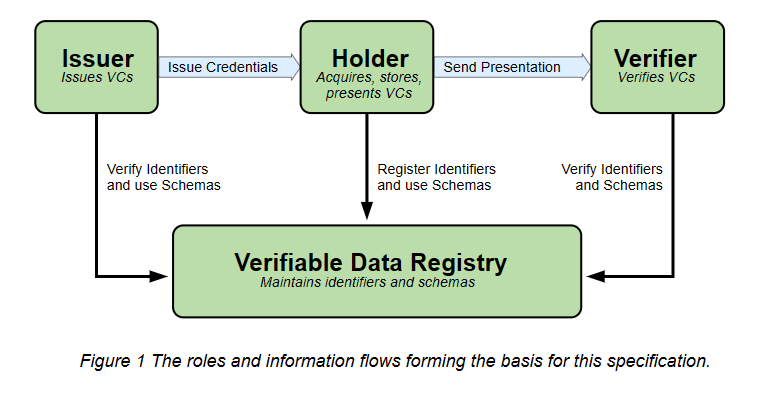
\includegraphics[scale = 1]{./res/images/Immaginew3c2.png}
\end{center}

\subsection{Presentazioni}
Il testo descrive l'importanza di migliorare la privacy come caratteristica fondamentale di questa specifica. Per fare ciò, si possono esprimere solo le parti rilevanti 
dell'identità di una persona in una presentazione verificabile. Questa presentazione contiene dati da una o più credenziali verificabili e garantisce l'autenticità delle informazioni. 
Le presentazioni verificabili possono aggregare dati provenienti da diversi emittenti e rappresentano un aspetto specifico di una persona, organizzazione o entità.
\begin{center}
	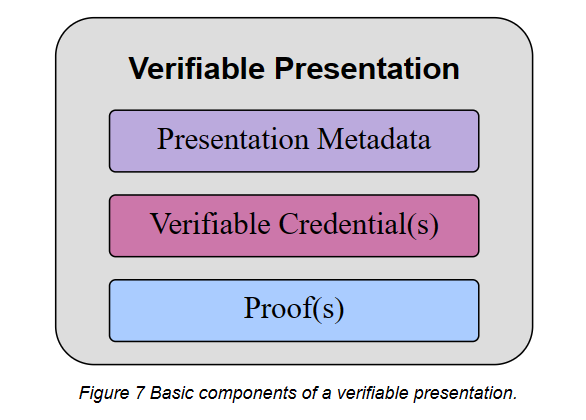
\includegraphics[scale = 1]{./res/images/Immaginew3c3.png}
\end{center}

\subsection{Ciclo di vita delle credenziali}
Il ciclo di vita delle credenziali e delle presentazioni nell'Ecosistema delle Credenziali Verificabili spesso segue un percorso comune:
\begin{itemize}
\item Emissione di una o più credenziali verificabili;
\item Conservazione delle credenziali verificabili in un repository delle credenziali (come un portafoglio digitale);
\item Composizione delle credenziali verificabili in una presentazione verificabile per i verificatori;
\item Verifica della presentazione verificabile da parte del verificatore.
\end{itemize}
\begin{center}
	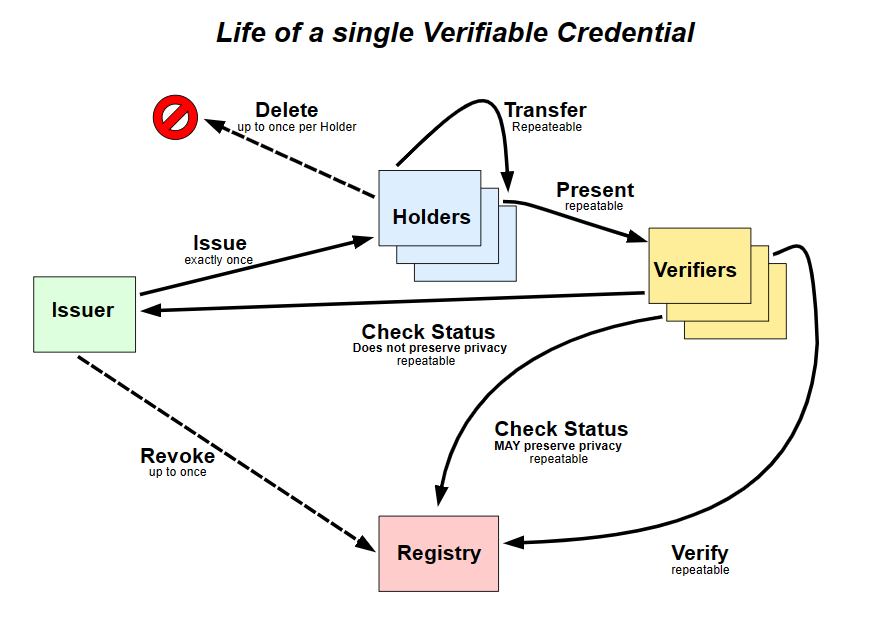
\includegraphics[scale = 1]{./res/images/Immaginew3c.png}
\end{center}

\subsection{Concetti base}
\begin{itemize}
\item \textbf{context}: Quando due sistemi software devono scambiare dati, devono utilizzare un linguaggio comprensibile da entrambi i sistemi.Questa specifica utilizza la proprietà \textit{@context}  per mappare tali alias brevi agli URI richiesti dalle specifiche credenziali verificabili e presentazioni verificabili.Le credenziali verificabili e le presentazioni verificabili 
DEVONO includere una proprietà \textit{@context}. Il valore della proprietà \textit{@context} DEVE essere un insieme ordinato in cui il primo elemento è un URI. Gli elementi successivi nell'array DEVONO esprimere informazioni di contesto e possono essere composti da qualsiasi combinazione di 
URI o oggetti. È RACCOMANDATO che ogni URI nel \textit{@context} sia un URI che, se dereferenziato, restituisce un documento contenente informazioni leggibili dalla macchina sul \textit{@context};

\item \textbf{identificatori}: La proprietà "\textit{id}" è destinata a fare riferimento in modo univoco a un oggetto, come una persona, un prodotto o un'organizzazione. Utilizzando la proprietà "\textit{id}", 
è possibile esprimere affermazioni su cose specifiche all'interno della credenziale verificabile.
Se la proprietà "\textit{id}" è presente:
La proprietà "\textit{id}" DEVE esprimere un identificatore che si prevede che gli altri utilizzino quando esprimono affermazioni su una cosa specifica identificata da quell'identificatore.
La proprietà "\textit{id}" NON DEVE avere più di un valore.
Il valore della proprietà "\textit{id}" DEVE essere un URI.
Il valore della proprietà "\textit{id}" DEVE essere un singolo URI. Si RACCOMANDA che l'URI nell'id sia un URI che, se dereferenziato, restituisce un documento contenente informazioni 
leggibili dalla macchina sull'\textit{id};

\item \textbf{tipi}: I sistemi software che elaborano i tipi di oggetti specificati in questo documento utilizzano le informazioni sul tipo per determinare se una credenziale verificabile o 
una presentazione verificabile fornita è appropriata. Questa specifica definisce una proprietà di tipo per l'espressione delle informazioni sul tipo.
Le credenziali verificabili e le presentazioni verificabili DEVONO avere una proprietà di tipo. Ciò significa che una credenziale o presentazione che non ha una proprietà di 
tipo non è verificabile e quindi non è né una credenziale verificabile né una presentazione verificabile.
Il valore della proprietà "\textit{type}" DEVE essere o mappare (attraverso l'interpretazione della proprietà "\textit{@context"}) a uno o più URI. Se vengono forniti più di un URI, gli URI DEVONO 
essere interpretati come un insieme non ordinato. Convenienze sintattiche DOVREBBERO essere utilizzate per facilitare l'uso da parte degli sviluppatori. Tali convenienze potrebbero 
includere termini JSON-LD. Si RACCOMANDA che ciascun URI nel tipo sia un URI che, se dereferenziato, restituisce un documento contenente informazioni leggibili dalla macchina sul tipo;

\item \textbf{credentialSubject}: Una credenziale verificabile contiene dichiarazioni su uno o più soggetti. Questa specifica definisce una proprietà "\textit{credentialSubject}" per 
l'espressione di dichiarazioni su uno o più soggetti.
Una credenziale verificabile DEVE avere una proprietà "\textit{credentialSubject}";

\item \textbf{issuer}: Questa specifica definisce una proprietà per esprimere l'emittente di una credenziale verificabile.
Una credenziale verificabile DEVE avere una proprietà "\textit{issuer}". Il valore della proprietà "\textit{issuer}" DEVE essere un URI o un oggetto contenente una proprietà "\textit{id}". Si RACCOMANDA 
che l'URI nell'emittente o nel suo id sia un URI che, se dereferenziato, restituisce un documento contenente informazioni leggibili dalla macchina sull'emittente che possono 
essere utilizzate per verificare le informazioni espresse nella credenziale;

\item \textbf{issuanceDate}: Questa specifica definisce la proprietà "\textit{issuanceDate}" per esprimere la data e l'ora in cui una credenziale diventa valida.
Una credenziale DEVE avere una proprietà "\textit{issuanceDate}". Il valore della proprietà "\textit{issuanceDate}" DEVE essere una stringa rappresentante una data e un'ora combinata che rappresenta la data e l'ora in cui la credenziale diventa valida, che potrebbe essere una data e un'ora future. Si noti che questo valore rappresenta il momento più presto 
in cui le informazioni associate alla proprietà "\textit{credentialSubject}" diventano valide;

\item \textbf{proof}: Uno o più proof crittografici che possono essere utilizzati per rilevare manomissioni e verificare l'autenticità di una credenziale o presentazione. 
Il metodo specifico utilizzato per una proof incorporata DEVE essere incluso utilizzando la proprietà "\textit{type}";

\item \textbf{expirationDate}: Questa specifica definisce la proprietà "\textit{expirationDate}" per l'espressione delle informazioni di scadenza della credenziale.
Se presente, il valore della proprietà "\textit{expirationDate}" DEVE essere una stringa rappresentante una data e un'ora che rappresenta la data e l'ora in cui la credenziale cessa 
di essere valida;

\item \textbf{status}: Questa specifica definisce la seguente proprietà "\textit{credentialStatus}" per la scoperta di informazioni sullo stato attuale di una credenziale verificabile, ad esempio 
se è sospesa o revocata.
\end{itemize}


\subsection{Esempi}
Un esempio di grande dataset:
\begin{itemize}
    \item un tipico caso di un grande dataset collegato è DBPedia, che, fondamentalmente, rende disponibile il contenuto di Wikipedia in formato RDF. L'importanza di DBPedia non è solo quella di includere i dati di Wikipedia, ma anche quella di incorporare collegamenti ad altri dataset sul Web, ad esempio a Geonames. Fornendo questi collegamenti aggiuntivi (sotto forma di triple RDF), le applicazioni possono sfruttare le conoscenze extra (e possibilmente più precise) provenienti da altri dataset durante lo sviluppo di un'applicazione; grazie all'integrazione di informazioni provenienti da diversi dataset, l'applicazione può offrire un'esperienza utente molto migliore.
\end{itemize}
Di seguito sono elencati alcuni esempi di come il W3C Data Model potrebbe essere applicato a un ipotetico portafoglio digitale che raccoglie le credenziali d'accesso degli utenti, come ad esempio il Sistema Pubblico di Identità Digitale (SPID):
\begin{itemize}
    \item \textbf{Rappresentazione delle credenziali}: utilizzando il W3C Data Model, il portafoglio digitale potrebbe rappresentare le credenziali d'accesso come oggetti RDF. Ad esempio, un oggetto RDF potrebbe rappresentare una specifica credenziale SPID con proprietà come "codice fiscale", "username", "password" e "scadenza";
    \item \textbf{Ontologia delle credenziali}: potrebbe essere utilizzata un'ontologia basata sul W3C Data Model per definire i concetti e le relazioni all'interno del portafoglio digitale. Questa ontologia potrebbe includere classi come "Credenziale", "Provider di Identità" e proprietà come "tipo di autenticazione" e "livello di affidabilità";
    \item \textbf{Annotazione semantica dei dati}: attraverso l'uso delle triple RDF, il portafoglio digitale potrebbe essere arricchito con metadati semantici per fornire ulteriori informazioni sulle credenziali. Ad esempio, potrebbero essere aggiunti metadati come "data di registrazione" o "ultima modifica" per tenere traccia delle attività relative alle credenziali;
    \item \textbf{Query e interrogazione}: utilizzando il linguaggio di interrogazione SPARQL, sarebbe possibile eseguire interrogazioni sulle credenziali nel portafoglio digitale. Ad esempio, si potrebbero recuperare tutte le credenziali associate a un determinato codice fiscale o controllare la validità di una specifica credenziale;
    \item \textbf{Esportazione e importazione dei dati}: il W3C Data Model consentirebbe l'esportazione e l'importazione dei dati del portafoglio digitale delle credenziali in diversi formati standard, come RDF/XML o Turtle. Ciò permetterebbe lo scambio dei dati con altri sistemi o applicazioni che utilizzano lo stesso modello di dati;
    \item \textbf{Privacy e sicurezza}: il W3C Data Model supporta anche questioni di privacy e sicurezza. Attraverso l'utilizzo di politiche di accesso controllato, crittografia e tecnologie di autenticazione, le credenziali sensibili nel portafoglio digitale potrebbero essere protette e accessibili solo agli utenti autorizzati;
    \item \textbf{Integrazione con servizi di autenticazione}: utilizzando il W3C Data Model, il portafoglio digitale potrebbe integrarsi con servizi di autenticazione basati su SPID o altri protocolli. Ad esempio, il portafoglio potrebbe fornire un'interfaccia per consentire all'utente di utilizzare le proprie credenziali SPID per l'autenticazione su piattaforme o applicazioni compatibili.
\end{itemize}

\subsection{Esempi di codice}
Per illustrare il ciclo di vita di una Verifiable Credential, useremo l'esempio del riscatto di uno sconto per ex studenti da parte di un'università. Nell'esempio seguente, Pat riceve una credenziale verificabile da ex studente da un'università e Pat memorizza la credenziale verificabile in un portafoglio digitale.\\

Un semplice esempio di una credenziale verificabile:
\begin{verbatim}
    {
  // set the context, which establishes the special terms we will be using
  // such as 'issuer' and 'alumniOf'.
  "@context": [
    "https://www.w3.org/2018/credentials/v1",
    "https://www.w3.org/2018/credentials/examples/v1"
  ],
  // specify the identifier for the credential
  "id": "http://example.edu/credentials/1872",
  // the credential types, which declare what data to expect in the credential
  "type": ["VerifiableCredential", "AlumniCredential"],
  // the entity that issued the credential
  "issuer": "https://example.edu/issuers/565049",
  // when the credential was issued
  "issuanceDate": "2010-01-01T19:23:24Z",
  // claims about the subjects of the credential
  "credentialSubject": {
    // identifier for the only subject of the credential
    "id": "did:example:ebfeb1f712ebc6f1c276e12ec21",
    // assertion about the only subject of the credential
    "alumniOf": {
      "id": "did:example:c276e12ec21ebfeb1f712ebc6f1",
      "name": [{
        "value": "Example University",
        "lang": "en"
      }, {
        "value": "Exemple d'Université",
        "lang": "fr"
      }]
    }
  },
  // digital proof that makes the credential tamper-evident
  // see the NOTE at end of this section for more detail
  "proof": {
    // the cryptographic signature suite that was used to generate the signature
    "type": "RsaSignature2018",
    // the date the signature was created
    "created": "2017-06-18T21:19:10Z",
    // purpose of this proof
    "proofPurpose": "assertionMethod",
    // the identifier of the public key that can verify the signature
    "verificationMethod": "https://example.edu/issuers/565049#key-1",
    // the digital signature value
    "jws": "eyJhbGciOiJSUzI1NiIsImI2NCI6ZmFsc2UsImNyaXQiOlsiYjY0Il19..TCYt5X
      sITJX1CxPCT8yAV-TVkIEq_PbChOMqsLfRoPsnsgw5WEuts01mq-pQy7UJiN5mgRxD-WUc
      X16dUEMGlv50aqzpqh4Qktb3rk-BuQy72IFLOqV0G_zS245-kronKb78cPN25DGlcTwLtj
      PAYuNzVBAh4vGHSrQyHUdBBPM"
  }
}
\end{verbatim}
Successivamente, Pat cerca di riscattare lo sconto per ex studenti. Il verificatore, un sistema di vendita di biglietti, afferma che ogni ex studente dell'"Example University" riceve uno sconto sui biglietti stagionali per gli eventi sportivi. Utilizzando un dispositivo mobile, Pat avvia il processo di acquisto di un abbonamento stagionale. Durante una fase di questo processo, viene richiesta una credenziale verificabile da ex studente, e questa richiesta viene inviata al portafoglio digitale di Pat. Il portafoglio digitale chiede a Pat se desidera fornire una credenziale verificabile precedentemente emessa. Pat seleziona la credenziale verificabile da ex studente, che viene quindi composta in una presentazione verificabile. La presentazione verificabile viene inviata al verificatore e viene verificata.\\

Un semplice esempio di una presentazione verificabile:
\begin{verbatim}
    {
  "@context": [
    "https://www.w3.org/2018/credentials/v1",
    "https://www.w3.org/2018/credentials/examples/v1"
  ],
  "type": "VerifiablePresentation",
  // the verifiable credential issued in the previous example
  "verifiableCredential": [{
    "@context": [
      "https://www.w3.org/2018/credentials/v1",
      "https://www.w3.org/2018/credentials/examples/v1"
    ],
    "id": "http://example.edu/credentials/1872",
    "type": ["VerifiableCredential", "AlumniCredential"],
    "issuer": "https://example.edu/issuers/565049",
    "issuanceDate": "2010-01-01T19:23:24Z",
    "credentialSubject": {
      "id": "did:example:ebfeb1f712ebc6f1c276e12ec21",
      "alumniOf": {
        "id": "did:example:c276e12ec21ebfeb1f712ebc6f1",
        "name": [{
          "value": "Example University",
          "lang": "en"
        }, {
          "value": "Exemple d'Université",
          "lang": "fr"
        }]
      }
    },
    "proof": {
      "type": "RsaSignature2018",
      "created": "2017-06-18T21:19:10Z",
      "proofPurpose": "assertionMethod",
      "verificationMethod": "https://example.edu/issuers/565049#key-1",
      "jws": "eyJhbGciOiJSUzI1NiIsImI2NCI6ZmFsc2UsImNyaXQiOlsiYjY0Il19..TCYt5X
        sITJX1CxPCT8yAV-TVkIEq_PbChOMqsLfRoPsnsgw5WEuts01mq-pQy7UJiN5mgRxD-WUc
        X16dUEMGlv50aqzpqh4Qktb3rk-BuQy72IFLOqV0G_zS245-kronKb78cPN25DGlcTwLtj
        PAYuNzVBAh4vGHSrQyHUdBBPM"
    }
  }],
  // digital signature by Pat on the presentation
  // protects against replay attacks
  "proof": {
    "type": "RsaSignature2018",
    "created": "2018-09-14T21:19:10Z",
    "proofPurpose": "authentication",
    "verificationMethod": "did:example:ebfeb1f712ebc6f1c276e12ec21#keys-1",
    // 'challenge' and 'domain' protect against replay attacks
    "challenge": "1f44d55f-f161-4938-a659-f8026467f126",
    "domain": "4jt78h47fh47",
    "jws": "eyJhbGciOiJSUzI1NiIsImI2NCI6ZmFsc2UsImNyaXQiOlsiYjY0Il19..kTCYt5
      XsITJX1CxPCT8yAV-TVIw5WEuts01mq-pQy7UJiN5mgREEMGlv50aqzpqh4Qq_PbChOMqs
      LfRoPsnsgxD-WUcX16dUOqV0G_zS245-kronKb78cPktb3rk-BuQy72IFLN25DYuNzVBAh
      4vGHSrQyHUGlcTwLtjPAnKb78"
  }
}
\end{verbatim}

Esempio e informazioni presi dal sito ufficiale del W3C:\\
\url{https://www.w3.org/TR/vc-data-model/#proof-formats}\\